\chapter{Конструкторская часть}

\section{Схема алгоритмов поиска расстояния Левенштейна}

На рисунках \ref{images:l_iterative_part1} и \ref{images:l_iterative_part2} представлена схема итеративного алгоритма вычисления расстояния Левенштейна, которая состоит из двух частей:

\begin{itemize}
\item на рисунке \ref{images:l_iterative_part1} показана первая часть,
\item на рисунке \ref{images:l_iterative_part2} — вторая часть.
\end{itemize}

\vspace{0.5cm}
На рисунке \ref{images:l_recursive} представлена схема рекурсивного алгоритма вычисления расстояния Левенштейна.

\vspace{0.5cm}
На рисунках \ref{images:l_recursive_cache_part1} и \ref{images:l_recursive_cache_part2} показана схема рекурсивного алгоритма с заполнением матрицы машинной бесконечностью, которая состоит из двух частей:

\begin{itemize}
\item на рисунке \ref{images:l_recursive_cache_part1} показана первая часть,
\item на рисунке \ref{images:l_recursive_cache_part2} — вторая часть.
\end{itemize}

\section{Схема алгоритма поиска расстояния Дамерау — Левенштейна}

На рисунках \ref{images:dl_part1} и \ref{images:dl_part2} представлена схема алгоритма вычисления расстояния Дамерау — Левенштейна, которая состоит из двух частей:

\begin{itemize}
\item на рисунке \ref{images:dl_part1} показана первая часть,
\item на рисунке \ref{images:dl_part2} — вторая часть.
\end{itemize}

\begin{figure}[H]
    \centering
    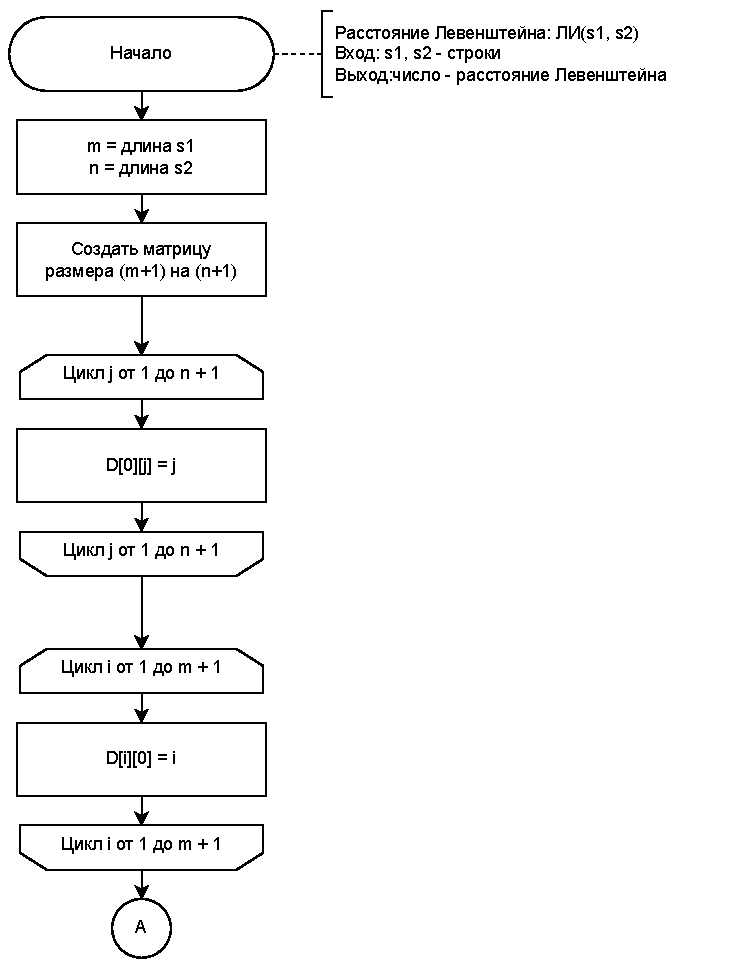
\includegraphics[width=150mm]{images/l_iterative_part1}
    \caption{Схема итеративного алгоритма вычисления расстояния Левенштейна. Часть 1.}
    \label{images:l_iterative_part1}
\end{figure}

\begin{figure}[H]
    \centering
    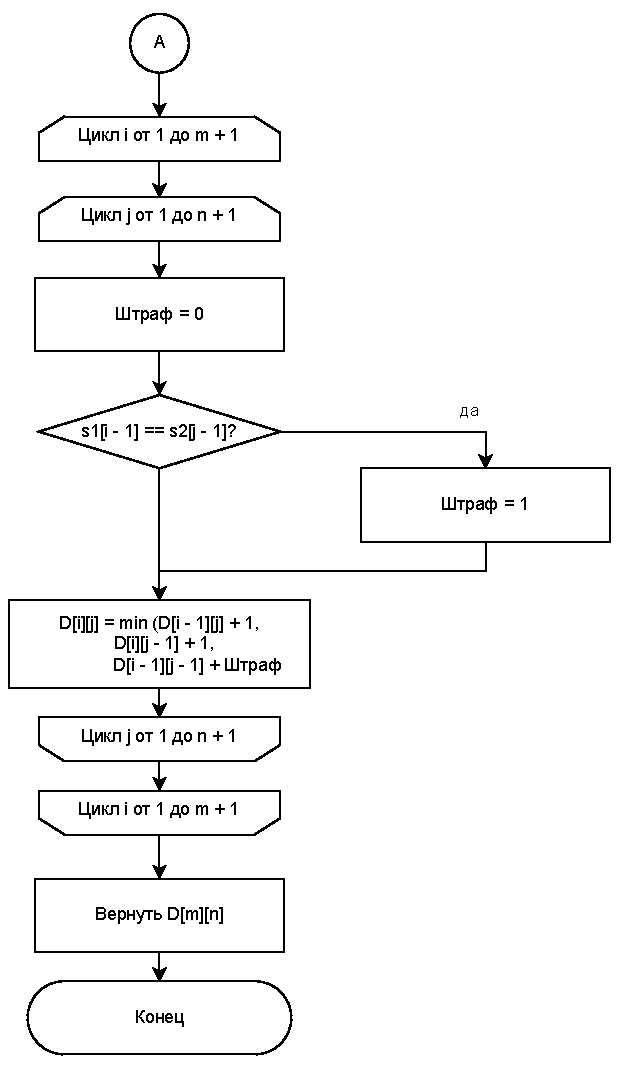
\includegraphics[width=130mm]{images/l_iterative_part2}
    \caption{Схема итеративного алгоритма вычисления расстояния Левенштейна. Часть 2.}
    \label{images:l_iterative_part2}
\end{figure}

\begin{figure}[H]
    \centering
    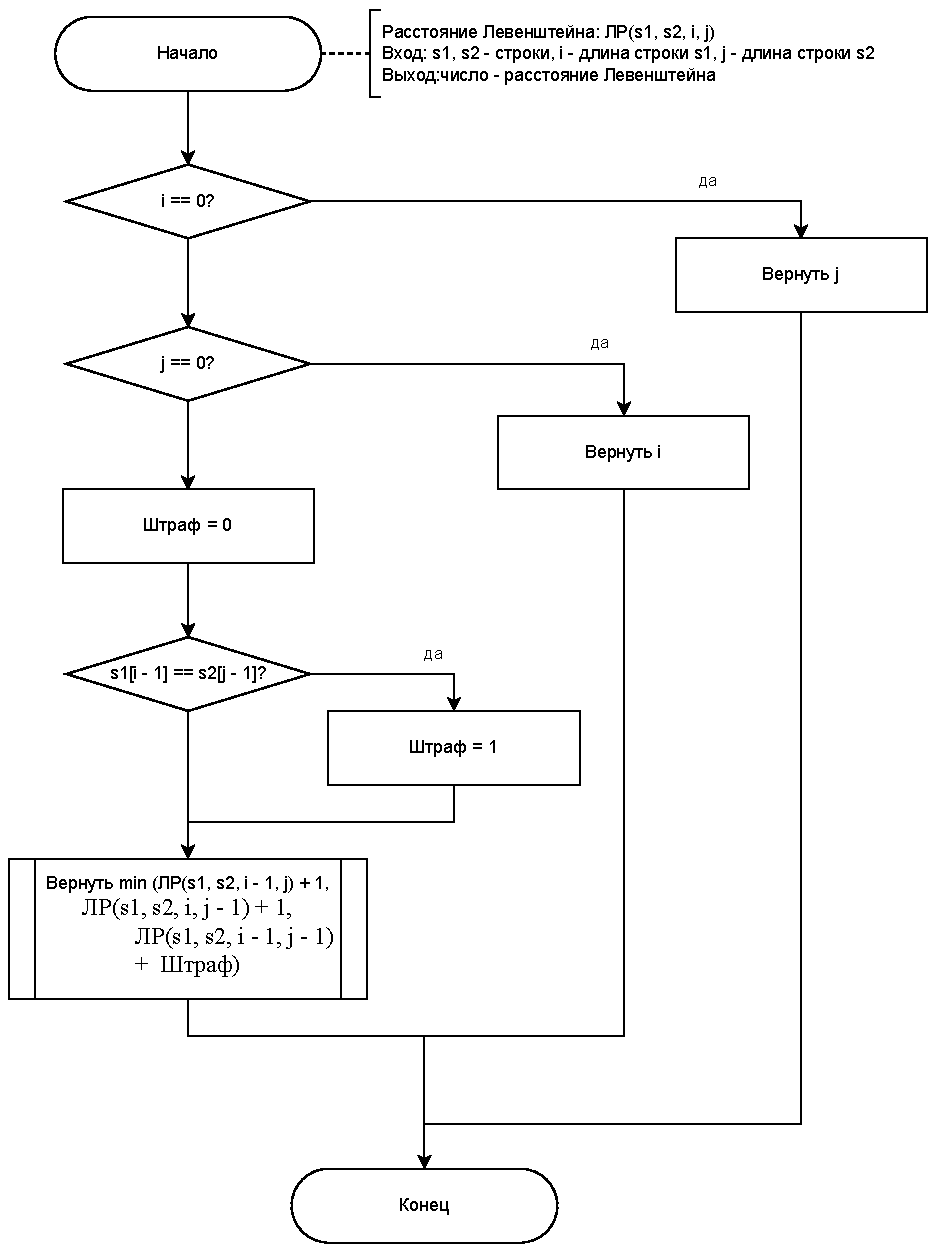
\includegraphics[width=170mm]{images/l_recursive}
    \caption{Схема рекурсивного алгоритма вычисления расстояния Левенштейна.}
    \label{images:l_recursive}
\end{figure}

\begin{figure}[H]
    \centering
    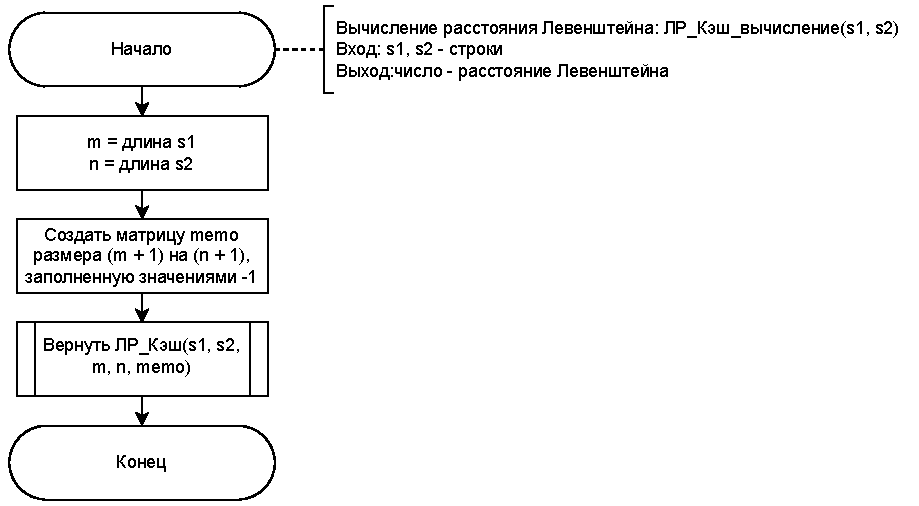
\includegraphics[width=170mm]{images/l_recursive_cache_part1}
    \caption{Схема рекурсивного алгоритма с заполнением матрицы. Часть 1.}
    \label{images:l_recursive_cache_part1}
\end{figure}

\begin{figure}[H]
    \centering
    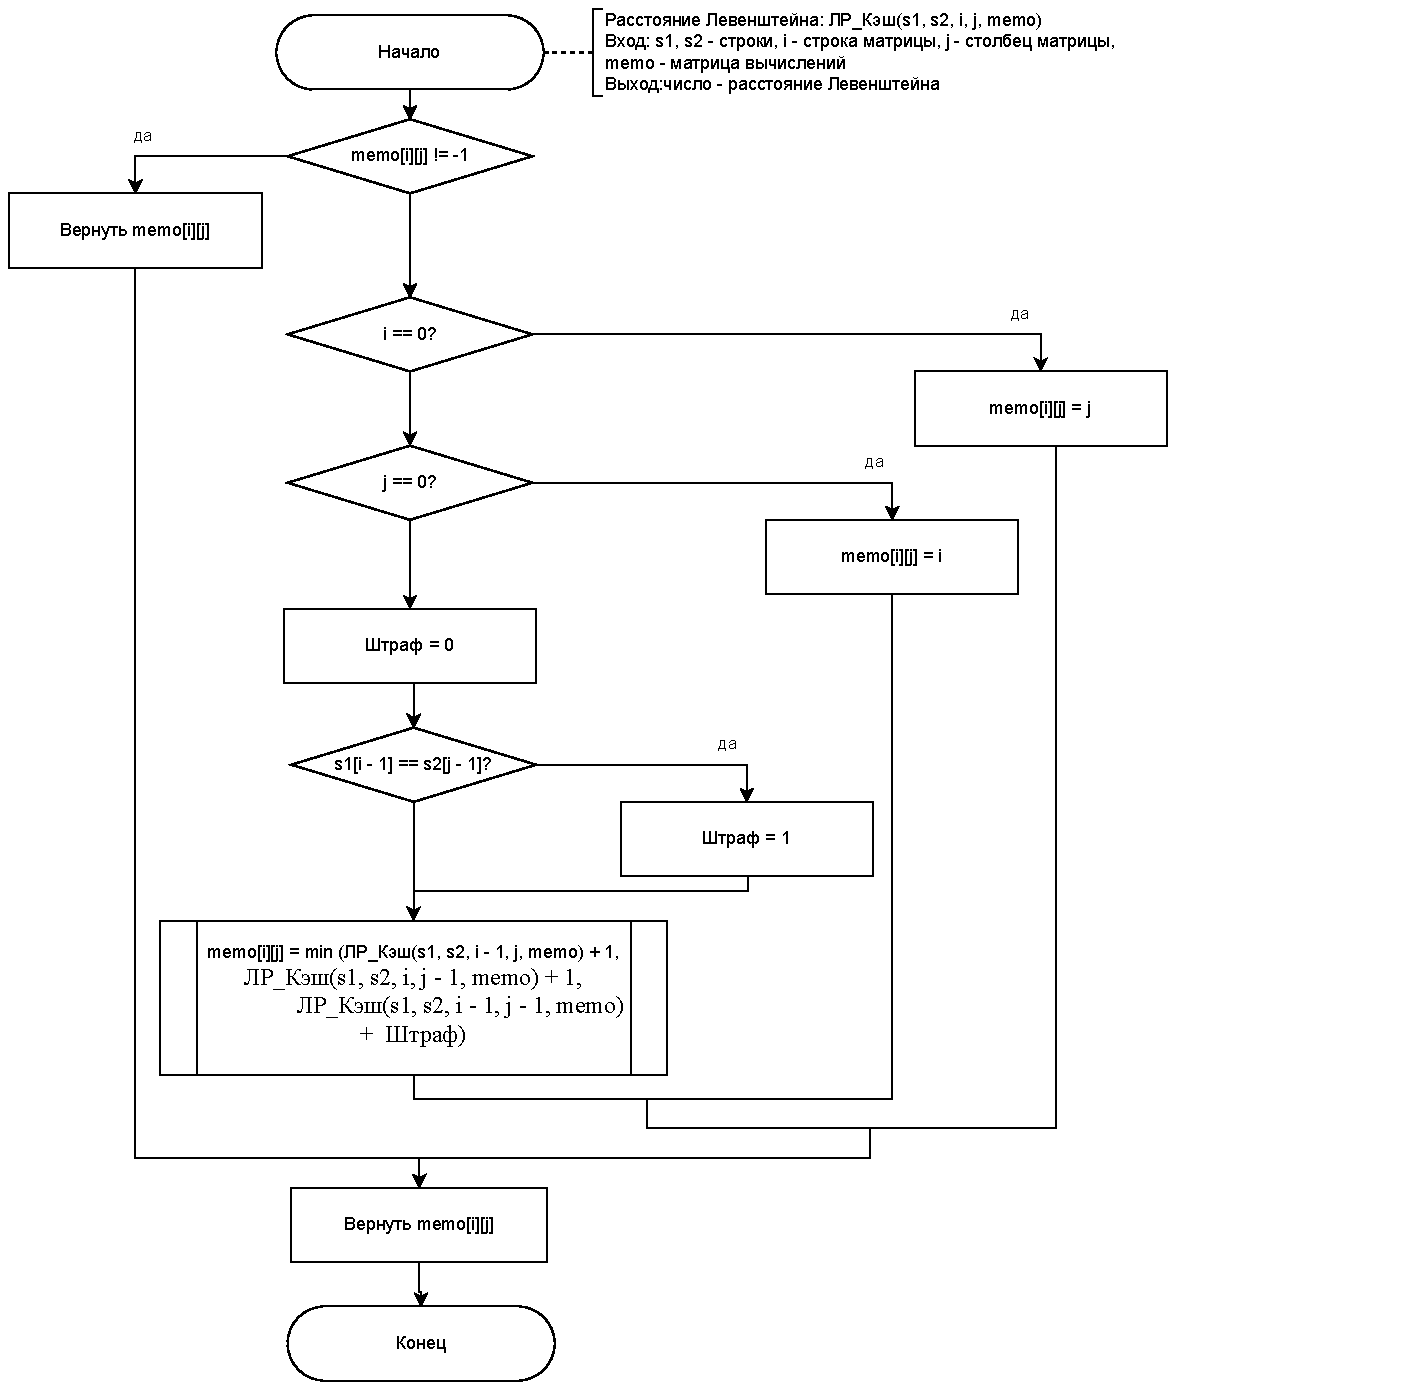
\includegraphics[width=185mm]{images/l_recursive_cache_part2}
    \caption{Схема рекурсивного алгоритма с заполнением матрицы. Часть 2.}
    \label{images:l_recursive_cache_part2}
\end{figure}

\begin{figure}[H]
    \centering
    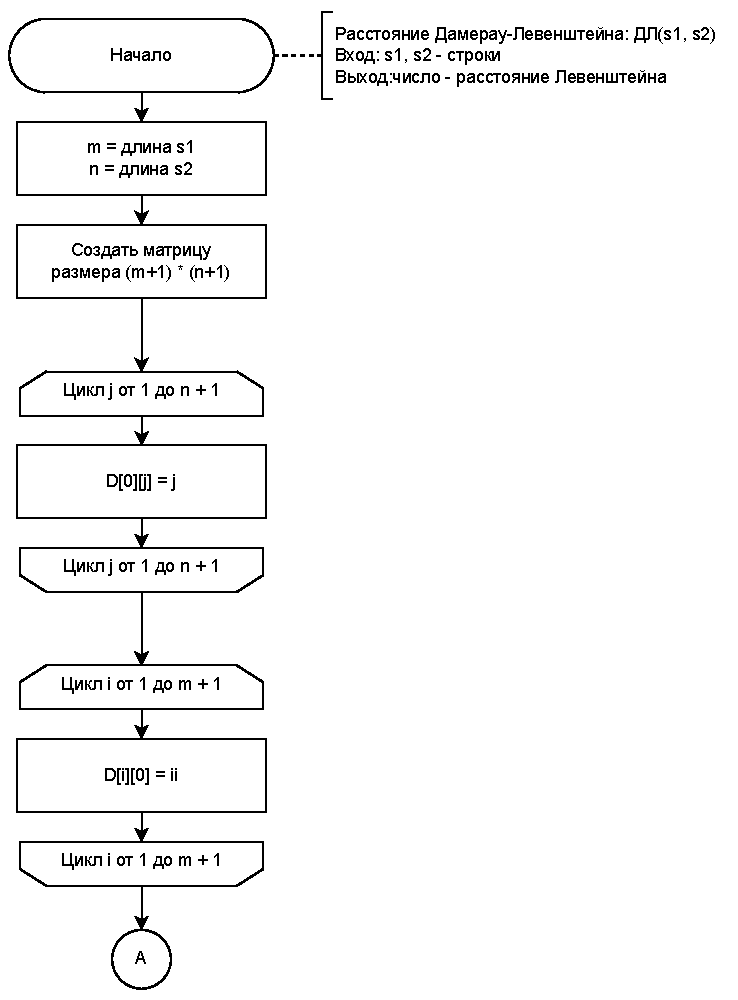
\includegraphics[width=170mm]{images/dl_part1}
    \caption{Схема алгоритма вычисления расстояния Дамерау — Левенштейна. Часть 1.}
    \label{images:dl_part1}
\end{figure}

\begin{figure}[H]
    \centering
    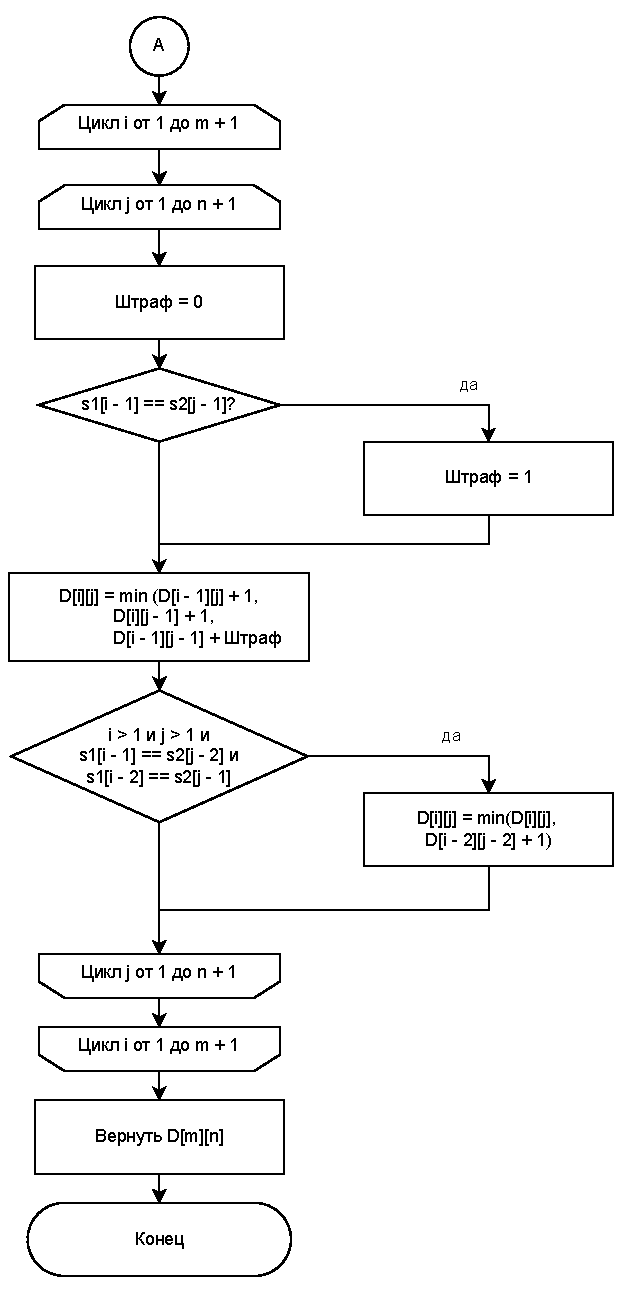
\includegraphics[width=120mm]{images/dl_part2}
    \caption{Схема алгоритма вычисления расстояния Дамерау — Левенштейна. Часть 2.}
    \label{images:dl_part2}
\end{figure}

\vspace{0.5cm}
\section*{Вывод}

На основе теоретических данных, полученных в аналитическом разделе, были разработаны схемы алгоритмов, необходимых для решения поставленных задач.